\documentclass[conference]{IEEEtran}

\usepackage{graphicx} % Required for inserting images
\usepackage{amsmath}
\usepackage[a4paper, margin=1.5cm]{geometry}
\usepackage{fancyhdr}
\usepackage{float}
\usepackage{booktabs}
\usepackage{caption}
\usepackage{subcaption}
\usepackage{hyperref}
\usepackage{siunitx}
\usepackage{wrapfig}
\usepackage{enumitem}
\usepackage{xcolor}
\usepackage{titlesec}
\usepackage{amssymb}
\usepackage{tabularx}
\usepackage{tikz}
\usetikzlibrary{positioning, arrows.meta}

% ====== Header configuration ======
\pagestyle{fancy}
\fancyhf{}
\fancyhead[L]{Research Assistant}
\renewcommand{\headrulewidth}{1pt}

% ====== Compact section spacing ======
\title{\vspace*{-3em}\fontsize{16}{18}\selectfont RNN Sentiment Analysis with Attention}
\titlespacing*{\section}{0pt}{2pt}{2pt}
\titlespacing*{\subsection}{0pt}{1.5pt}{1.5pt}

\title{Research Assistant}
\author{\IEEEauthorblockN{Nuria Balbás, Ana Pascual, Cristina Sobrino}}
\date{April 2026}

\begin{document}
\maketitle

% ===========================
% MAIN SECTIONS
% ===========================

\section{System Design}

\begin{figure}[H]
\centering
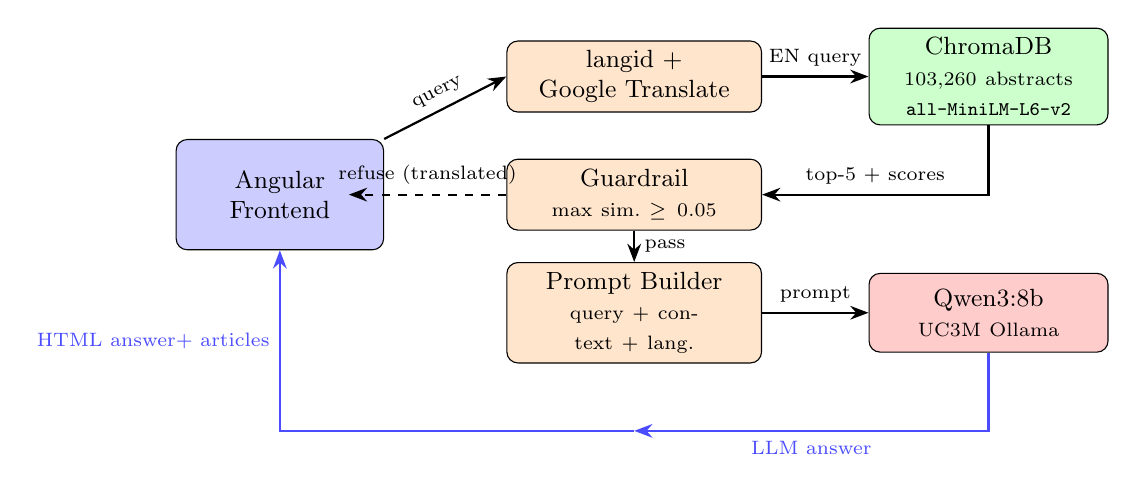
\begin{tikzpicture}[
    fe/.style={rectangle, draw, rounded corners=4pt, fill=blue!20,
               text width=2.4cm, minimum height=1.4cm, align=center, font=\small},
    be/.style={rectangle, draw, rounded corners=4pt, fill=orange!20,
               text width=3.0cm, minimum height=0.9cm, align=center, font=\small},
    db/.style={rectangle, draw, rounded corners=4pt, fill=green!20,
               text width=2.8cm, minimum height=1.2cm, align=center, font=\small},
    lm/.style={rectangle, draw, rounded corners=4pt, fill=red!20,
               text width=2.8cm, minimum height=1.0cm, align=center, font=\small},
    arr/.style={-{Stealth}, thick},
    ret/.style={-{Stealth}, thick, color=blue!70}
]

\node[fe] (ui)     at (0, 0)     {Angular\\Frontend};
\node[be] (lang)   at (4.5, 1.5) {langid +\\Google Translate};
\node[db] (chroma) at (9, 1.5)   {ChromaDB\\{\scriptsize 103{,}260 abstracts}\\{\scriptsize\texttt{all-MiniLM-L6-v2}}};
\node[be] (guard)  at (4.5, 0)   {Guardrail\\{\scriptsize max sim.\ $\geq 0.05$}};
\node[be] (prompt) at (4.5,-1.5) {Prompt Builder\\{\scriptsize query + context + lang.}};
\node[lm] (llm)    at (9, -1.5)  {Qwen3:8b\\{\scriptsize UC3M Ollama}};

\draw[arr] (ui.north east) -- node[above,font=\scriptsize,sloped]{query} (lang.west);
\draw[arr] (lang)          -- node[above,font=\scriptsize]{EN query} (chroma);
\draw[arr] (chroma.south)  -- (9,0) -- node[above,font=\scriptsize]{top-5 + scores} (guard.east);
\draw[arr] (guard)         -- node[right,font=\scriptsize]{pass} (prompt);
\draw[arr] (prompt)        -- node[above,font=\scriptsize]{prompt} (llm);
\draw[arr,dashed] (guard.west) -- node[above,font=\scriptsize]{refuse (translated)} ++(-2,0);
% LLM answer returns to backend, then backend sends full response to frontend
\draw[ret] (llm.south) -- (9,-3) -- node[below,font=\scriptsize]{LLM answer} (4.5,-3);
\draw[ret] (4.5,-3)    -- (0,-3) -- node[left,font=\scriptsize]{HTML answer\\+ articles} (ui.south);

\end{tikzpicture}
\caption{System architecture. \textcolor{blue!80}{Blue}: frontend; \textcolor{orange!80}{orange}: backend; \textcolor{green!60!black}{green}: vector store; \textcolor{red!70}{red}: LLM. Blue return arrow shows the response path.}
\label{fig:architecture}
\end{figure}

The backend is a Python service that exposes the RAG pipeline as two HTTP endpoints (\texttt{/search} and \texttt{/summarize}) over FastAPI. We chose arXiv as our document source because it spans every research area we expected users to ask about, its metadata is openly redistributable, and the title plus abstract is enough to retrieve and compare ideas without parsing full PDFs. From the public arXiv dump we filtered \textbf{103{,}260} papers, keeping only entries with all required fields populated, dropping abstracts shorter than 50 characters, and deduplicating on both \texttt{id} and \texttt{(title, abstract)}.

We use ChromaDB as the vector store: it persists locally, has a Python-native API, and ships with HNSW-based approximate retrieval, so we did not need to run a separate vector server. The remote LLM is reached through the UC3M Ollama gateway with a thin client wrapper.

On top of the mandatory functional requirements we implemented three additional features. (i)~\textbf{Multilingual support.} The query language is detected with \texttt{langid}; non-English queries are translated to English for retrieval (the embedding model is English-only) but the original query and the detected language are passed to the LLM, which is instructed to answer in the user's language. (ii)~\textbf{On-demand article summaries} via \texttt{/summarize}, triggered per article from the frontend so the user only pays the LLM cost for papers they actually open. (iii)~\textbf{Evaluation mode.} A request flag enables a parallel exact nearest-neighbour (ENN) search over all 103k embeddings and returns ANN-vs-ENN recall and per-stage timing alongside the answer, exposing the approximation tradeoff directly to the user.


\section{Configuration and Optimization}

\textbf{Vector database.} Each document indexed in ChromaDB is the concatenation \texttt{"Title: ...\textbackslash nAbstract: ..."}, embedded with \texttt{all-MiniLM-L6-v2} (384-dim sentence-transformer). We embed title and abstract together because in spot checks many papers carried the topic words only in the title; authors, categories, and update date are stored as metadata so the frontend can display them without polluting the embedding. Documents are inserted in batches of 1{,}000. Retrieval uses HNSW (Chroma's default ANN index) with $k=5$, and we expose the similarity score $s = 1 - d$ (with $d$ the L2 distance) to both the frontend and the guardrail.

\textbf{LLM.} We use \texttt{qwen3:8b} served by Ollama on the UC3M GPU. Among the three available models we picked Qwen3 over \texttt{llama3.1:8b} for its substantially better multilingual coverage (which we need for Spanish, French, Italian and German queries) and over \texttt{gemma3:4b} for the extra capacity needed by our long, structured output. Temperature is set to \textbf{0.0}: the task is grounded comparison, not creative generation, and determinism makes the system reproducible for evaluation. Other generation parameters are left at Ollama defaults; tuning them gave no measurable benefit.

\textbf{Prompting.} Anti-hallucination is split between a system prompt and a task prompt. The system prompt forces the response language and forbids adding information outside the context. The comparison prompt repeats and tightens these rules: only use the provided context, do not invent articles, methods, datasets or results, and explicitly state when the context is insufficient. It also fixes the output structure (\emph{research direction $\rightarrow$ relevant articles $\rightarrow$ key differences $\rightarrow$ possible novelty $\rightarrow$ conclusion}) and asks for HTML fragments, which the Angular frontend renders directly through \texttt{[innerHTML]}.

\textbf{Guardrail.} Prompting alone does not stop the model from confidently comparing the user's idea against weakly relevant papers. We therefore reject low-confidence queries before any LLM call: if the maximum retrieval similarity is below \textbf{0.05}, the backend returns a fixed refusal (translated back into the user's language) and skips generation entirely. The threshold was chosen by inspection of off-topic probes --- at this level genuinely unrelated queries are rejected while loosely related ones still receive a response.

\textbf{Innovation: dual ANN/ENN retrieval.} When \texttt{eval\_mode} is enabled, the backend runs the production HNSW search and a brute-force scan over the full embedding matrix, then returns both result lists, ANN/ENN timings, and the recall of ANN against ENN. This lets us quantify the cost of the approximation rather than assume it is negligible.

\section{System Evaluation}

We evaluate the system against the three criteria in the project brief. Retrieval quality is measured with Precision@$k$ over a manually curated set of 10 scenarios spanning clear matches, borderline topics, off-topic probes, and a single-token edge case, with binary relevance assigned at a similarity threshold of 0.35 (the empirical boundary between clearly and weakly relevant retrievals in our scenarios). We complement this with RAGAS Faithfulness using Llama-3.3-70B as the judge, which scores how grounded the generated answer is in the retrieved abstracts. Document coverage is the fraction of test queries whose top retrieval clears the 0.05 guardrail. Response time is decomposed into ANN retrieval and LLM generation, since the two have very different variance profiles.

\begin{table}[htpb]
    \centering
    \caption{System Evaluation for the Research Assistance Application.}
    \label{tab:system_evaluation}
    \renewcommand{\arraystretch}{1.3} % Añade un poco de espacio entre filas para mayor claridad
    \begin{tabularx}{\textwidth}{@{} l X l X @{}}
        \toprule
        \textbf{Criterion} & \textbf{Description} & \textbf{Measured Metric} & \textbf{Result} \\
        \midrule
        
        \textbf{RAG System Quality} &
        Retrieves key articles and accurately compares them with prior research. &
        Precision@5 (sim.\ threshold 0.35) over 10 scenarios; RAGAS Faithfulness with Llama-3.3-70B judge. &
        \textbf{0.68} mean P@5; \textbf{[TODO: Faithfulness]} \\

        \textbf{Document Coverage} &
        Ability to retrieve relevant articles related to the research topic. &
        \% of test queries with at least one retrieved article above the 0.05 guardrail. &
        \textbf{[TODO: \%]} over \textbf{[TODO: N]} queries \\

        \textbf{Response Time} &
        Speed of article retrieval and comparison generation. &
        Mean end-to-end latency, split into ANN retrieval and LLM generation. &
        \textbf{[TODO: ANN ms]} retrieval + \textbf{[TODO: s]} LLM \\
        
        \bottomrule
    \end{tabularx}
\end{table}

\section{Limitations}

\textbf{General-purpose embeddings.} \texttt{all-MiniLM-L6-v2} is trained on web text, not academic abstracts, so retrieval can miss domain-specific synonyms (e.g., ``GAN'' vs.\ ``generative adversarial network''). A science-domain encoder such as SPECTER or SciNCL would likely raise recall on technical queries, at the cost of larger embeddings and slower indexing.

\textbf{Translation is a silent failure mode.} Non-English queries pass through Google Translate before retrieval, and mistranslations of technical terms degrade retrieval without surfacing any error: the LLM still receives a fluent English query, but anchored to the wrong topic.

\textbf{Heuristic guardrail.} The 0.05 threshold was tuned by inspection rather than calibrated against a labelled relevance set. Broad-but-irrelevant queries can still pass it, after which the LLM dutifully compares the user's idea to weakly related papers. A learned classifier over the score distribution would be a more principled choice.

\textbf{Hallucinations are constrained, not eliminated.} The strict prompt and temperature 0 reduce fabrication, but the model still occasionally drifts when paraphrasing thin context (one or two retrieved abstracts above the threshold). The drift is small --- usually overgeneralising what an abstract claims --- but it is the residual failure mode we observed most often.

\textbf{Shared LLM infrastructure.} The Ollama server is shared across teams. End-to-end latency therefore has a variance component we cannot control, and a few requests during peak hours took several times the median time.

\section{Conclusions}

We built a multilingual academic research assistant grounded on 103k arXiv abstracts. The combination of a similarity-based guardrail, strict context-only prompting, and a deterministic LLM keeps the system honest about what it does and does not know, while ChromaDB with HNSW gives sub-second retrieval over the full corpus. The optional ENN mode lets us quantify the recall lost to approximation rather than assume it. The clearest next steps are switching to a science-domain embedding model, calibrating the guardrail threshold on a labelled set, and caching repeated queries to absorb LLM-server latency variance.


\end{document}


